\documentclass{article}

\usepackage{geometry}
\usepackage{graphicx}
\usepackage{booktabs}
\usepackage{makecell}
\usepackage{amsthm,amsmath,amsfonts}

\title{Additional file 1 --- Operating characteristcs for other accrual scenarios}
\date{}

%%% Begin ...
\begin{document}
\maketitle

\section{Constant accrual of 5 participants per week}

This section presents the trial operating characteristics assuming a slow than anticpated accrual of 5 participants per week.

\begin{table}[!ht]
	\footnotesize
	\caption{\label{tab:oc1}Trial operating characteristics assuming constant accrual of 5 per week, where $q=0.95$, $\underline{c}=0.05$, and $\overline{c}=0.95$.}
	\centering
	\begin{tabular}[t]{lrrrrrrrrr}
	\toprule
	$\theta_a^\star$ & $\theta_w^\star$ & \makecell{Decide\\superior} & \makecell{Stop\\early\\superior} & \makecell{No\\stop\\superior} & \makecell{Stop\\futile} & \makecell{Stop\\expect\\success} & \makecell{Superior\\following\\futile} & \makecell{Superior\\following\\exepct\\success} & \makecell{Expected\\sample\\size}\\
	\midrule
	0.10 & 0.05 & 0.98 & 0.97 & 0.00 & 0.01 & 0.99 & 0.07 & 0.99 & 1014\\
	     & 0.06 & 0.95 & 0.93 & 0.02 & 0.02 & 0.95 & 0.02 & 0.98 & 1305\\
	     & 0.07 & 0.83 & 0.73 & 0.10 & 0.10 & 0.76 & 0.00 & 0.96 & 1676\\
	     & 0.08 & 0.56 & 0.44 & 0.13 & 0.29 & 0.46 & 0.00 & 0.94 & 1933\\
	     & 0.09 & 0.24 & 0.16 & 0.08 & 0.59 & 0.19 & 0.00 & 0.86 & 1865\\
	     & 0.10 & 0.07 & 0.05 & 0.02 & 0.84 & 0.06 & 0.00 & 0.81 & 1574\\
	\bottomrule
	\end{tabular}
\end{table}

\begin{figure}[!ht]
	\caption{Probability of deciding superiority at the final analysis by decision thresholds and effect size assuming constant 5 per week accrual.}
	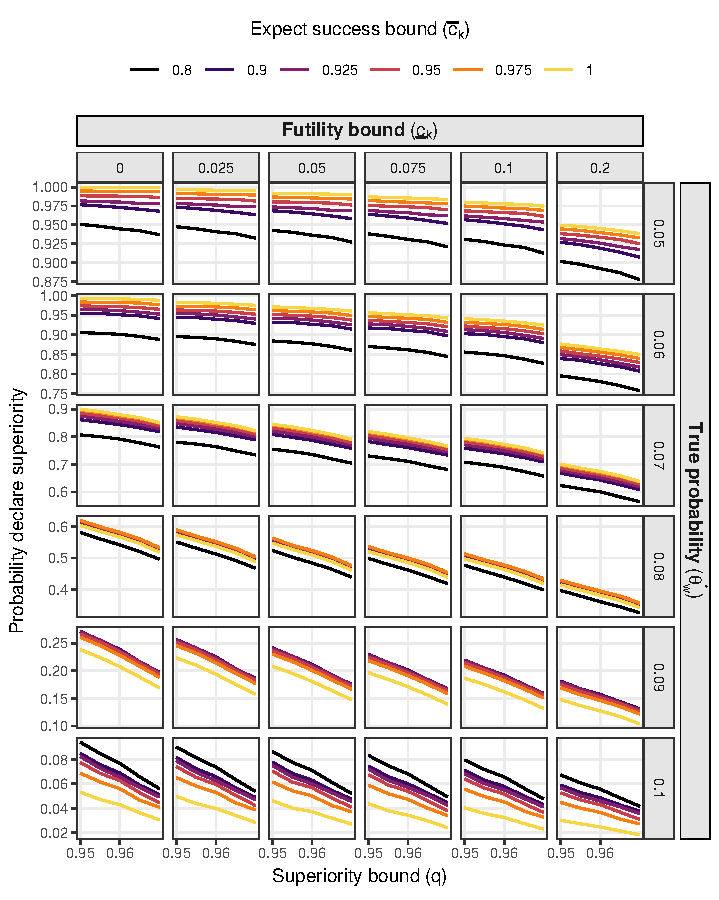
\includegraphics{figures/superiority_5.pdf}
	\label{fig:superiority_5}
\end{figure}

\begin{figure}[!ht]
	\caption{Expected sample size by decision thresholds and effect size assuming constant 5 per week accrual.}
	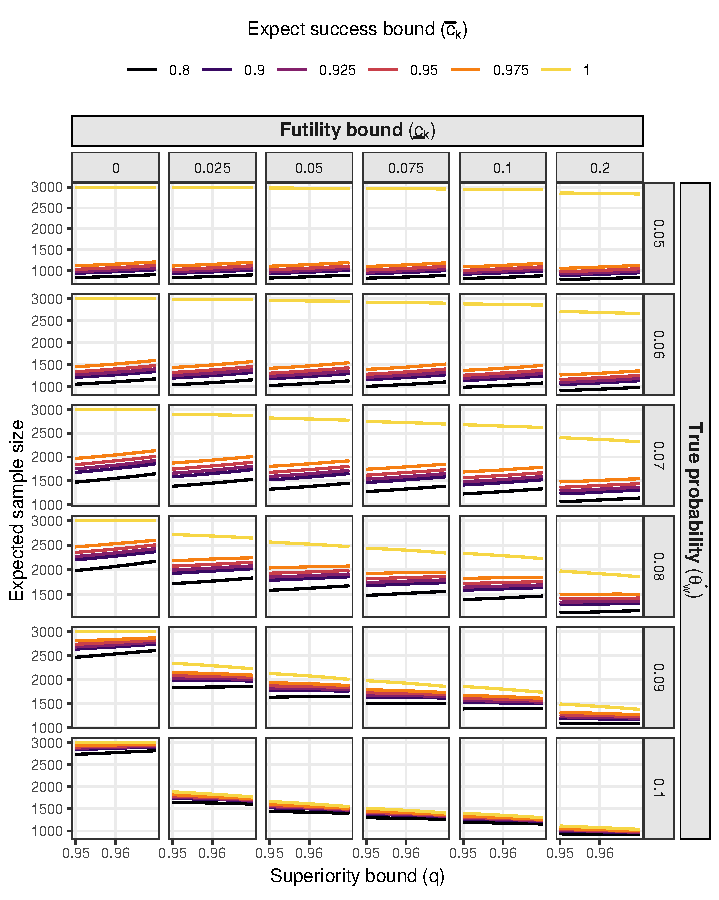
\includegraphics{figures/expected_ss_5.pdf}
	\label{fig:expected_ss_5}
\end{figure}

\begin{figure}[!ht]
	\caption{Marginal stopping probability for expected success by stage, effect size, and thresholds assuming constant 5 per week accrual and futility bound $\underline{c}=0.05$.}
	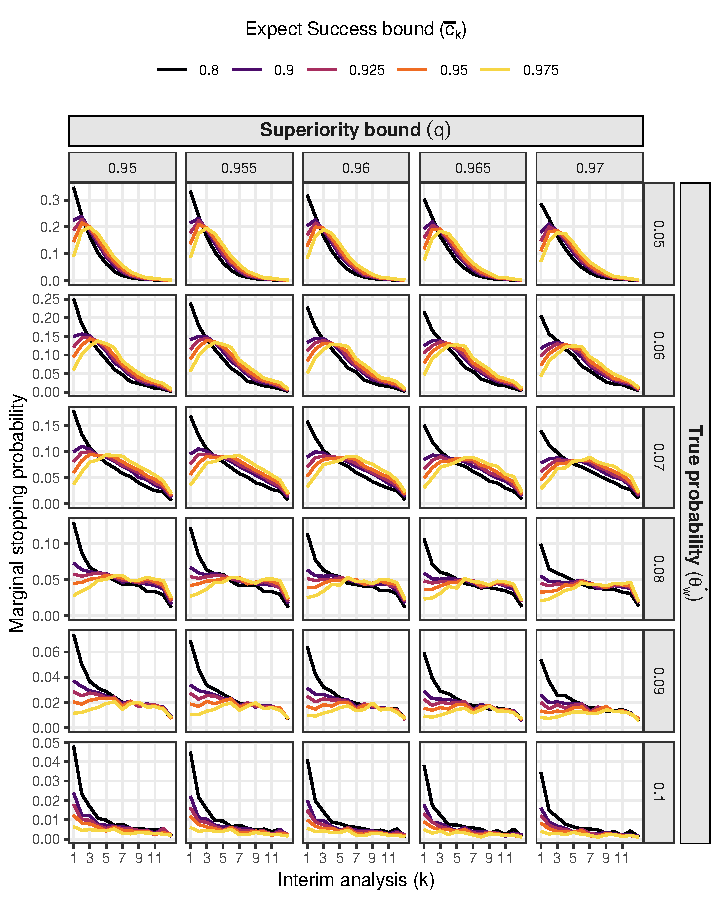
\includegraphics{figures/stop_expect_success_5.pdf}
	\label{fig:stop_expect_success_5}
\end{figure}

\begin{figure}[!ht]
	\caption{Marginal stopping probability for futility by stage, effect size, and thresholds assuming constant 5 per week accrual and expected success bound $\overline{c}=0.95$.}
	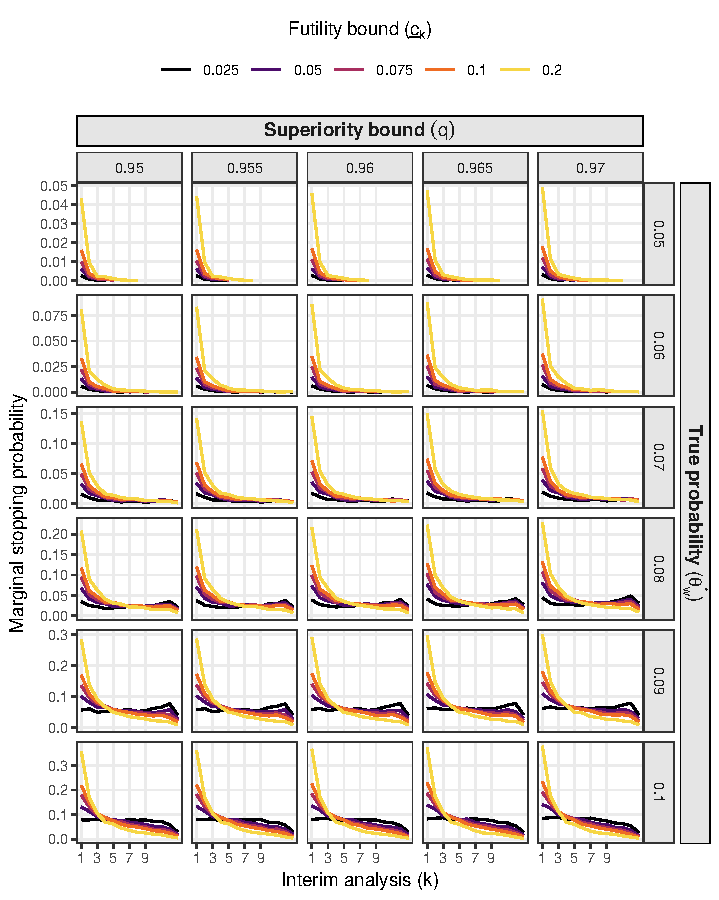
\includegraphics{figures/stop_futility_5.pdf}
	\label{fig:stop_futility_5}
\end{figure}

\clearpage

\section{Ramp-up of accrual over time}

This section presents the trial operating characteristics assuming a ramp-up in accrual over time.
Initially, it is assumed that accrual is slow over the first 12 months of the study before gradually increasing to a fixed accrual rate after 3 years.

\begin{table}[!ht]
	\footnotesize
	\caption{\label{tab:oc1}Trial operating characteristics assuming a ramp-up of accrual over time, where $q=0.95$, $\underline{c}=0.05$, and $\overline{c}=0.95$.}
	\centering
	\begin{tabular}[t]{lrrrrrrrrr}
	\toprule
	$\theta_a^\star$ & $\theta_w^\star$ & \makecell{Decide\\superior} & \makecell{Stop\\early\\superior} & \makecell{No\\stop\\superior} & \makecell{Stop\\futile} & \makecell{Stop\\expect\\success} & \makecell{Superior\\following\\futile} & \makecell{Superior\\following\\exepct\\success} & \makecell{Expected\\sample\\size}\\
	\midrule
	0.10 & 0.05 & 1.00 & 0.91 & 0.09 & 0.01 & 0.90 & 0.76 & 1.00 & 1985 \\
	     & 0.06 & 0.97 & 0.72 & 0.25 & 0.02 & 0.72 & 0.52 & 0.99 & 2267 \\
	     & 0.07 & 0.86 & 0.45 & 0.41 & 0.07 & 0.46 & 0.25 & 0.95 & 2479 \\
	     & 0.08 & 0.56 & 0.21 & 0.35 & 0.17 & 0.24 & 0.09 & 0.83 & 2586 \\
	     & 0.09 & 0.23 & 0.07 & 0.16 & 0.35 & 0.10 & 0.02 & 0.63 & 2534 \\
	     & 0.10 & 0.05 & 0.02 & 0.03 & 0.57 & 0.04 & 0.01 & 0.36 & 2361 \\
	\bottomrule
	\end{tabular}
\end{table}


\begin{figure}[!ht]
	\caption{Probability of deciding superiority at the final analysis by decision thresholds and effect size assuming ramp-up accrual.}
	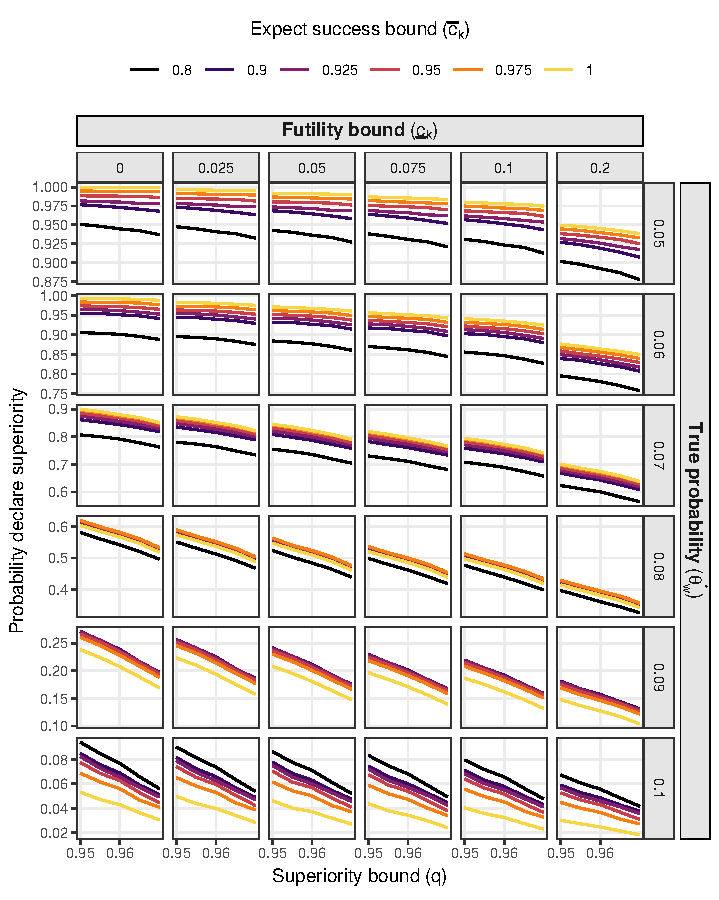
\includegraphics{figures/superiority_5.pdf}
	\label{fig:superiority_rampup}
\end{figure}

\begin{figure}[!ht]
	\caption{Expected sample size by decision thresholds and effect size assuming ramp-up accrual.}
	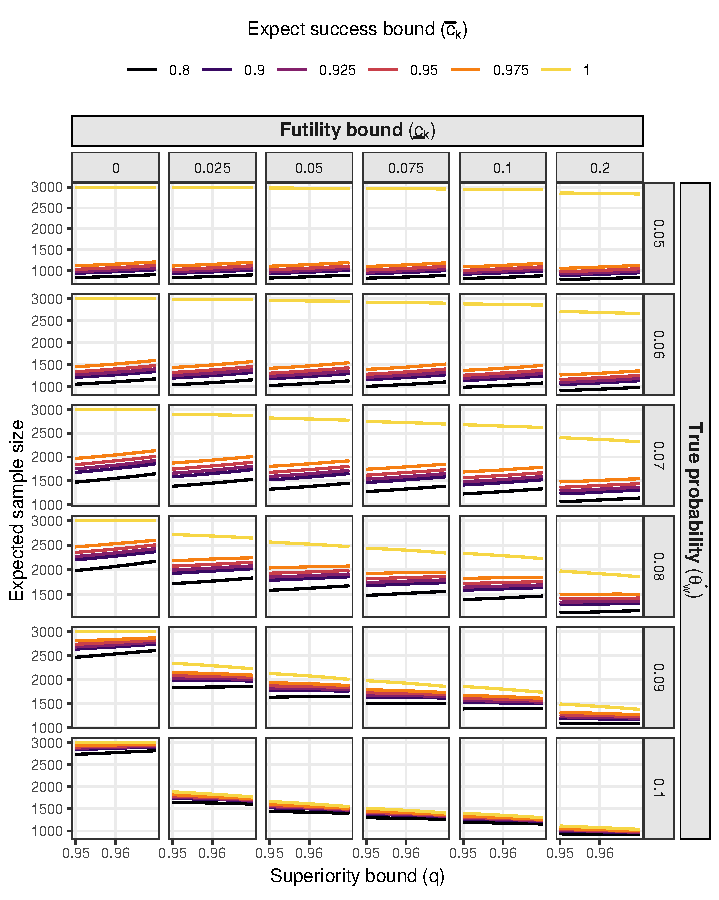
\includegraphics{figures/expected_ss_5.pdf}
	\label{fig:expected_ss_rampup}
\end{figure}

\begin{figure}[!ht]
	\caption{Marginal stopping probability for expected success by stage, effect size, and thresholds assuming ramp-up accrual and futility bound $\underline{c}=0.05$.}
	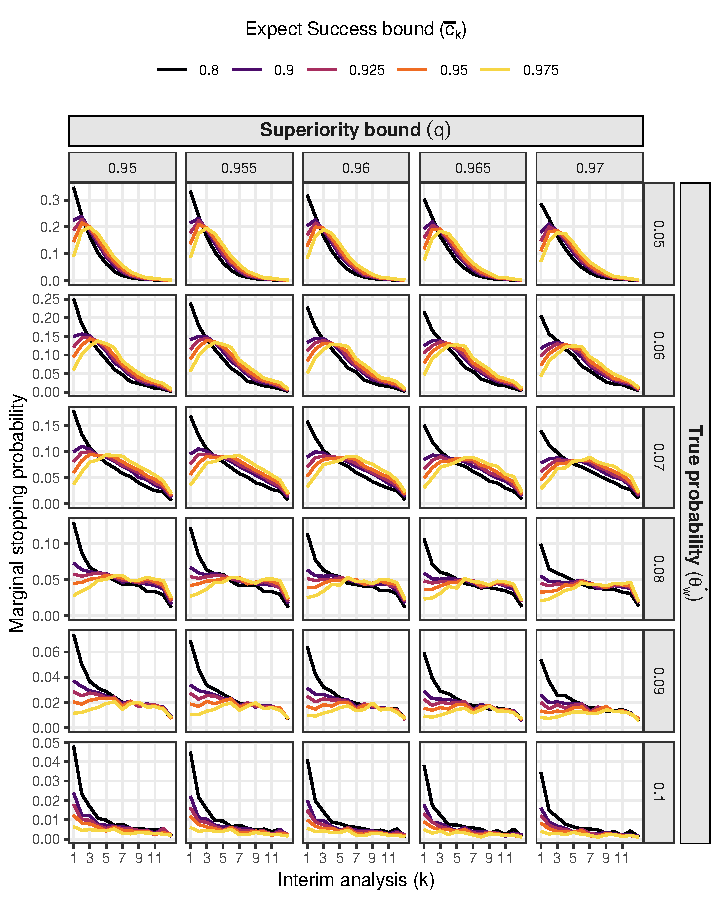
\includegraphics{figures/stop_expect_success_5.pdf}
	\label{fig:stop_expect_success_rampup}
\end{figure}

\begin{figure}[!ht]
	\caption{Marginal stopping probability for futility by stage, effect size, and thresholds assuming ramp-up accrual and expected success bound $\overline{c}=0.95$.}
	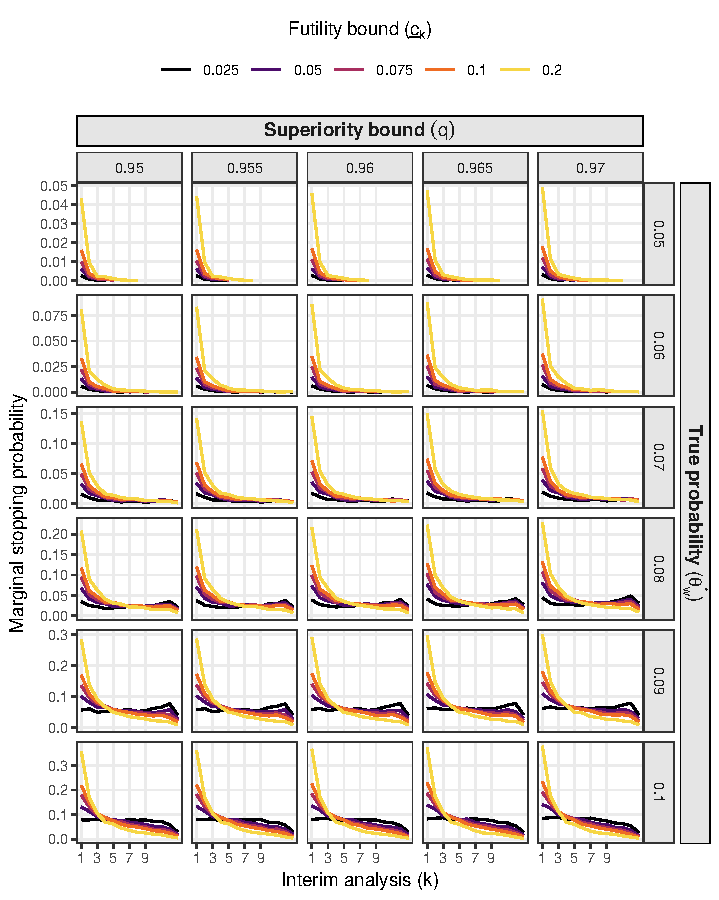
\includegraphics{figures/stop_futility_5.pdf}
	\label{fig:stop_futility_rampup}
\end{figure}


\end{document}